\chapter{Related Work} \label{cpt-related-work}

The approach we are proposing is an aggregation of a lot of ideas and implementations that have been 
around for quite some time. It is of great interest to explore related work which can provide 
context for use cases and additional techniques. Since our implementation is based on the areas 
of Voxel Redering, Occlusion Culling and Mesh Shading, this chapter will highlight related work 
for each of these topics.

[@TODO: Check redundancy with technological background]

\section{Voxel Representation} \label{sec-voxel-representation}

\begin{figure}[h]
    \centering
    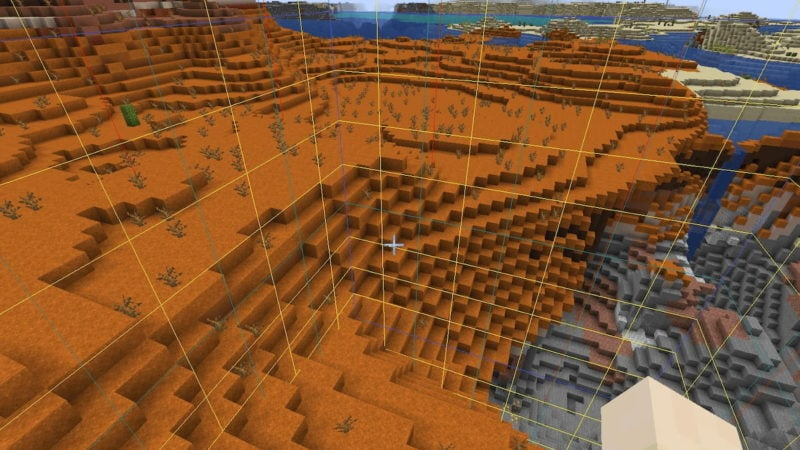
\includegraphics[width=300px]{images/graphics/minecraft-chunks.jpg}
    \caption{A screenshot from \emph{Minecraft}, with a debug visualization of the voxel chunks \cite{Palm2022}.}
    \label{fig:minecraft-chunks}
\end{figure}

\noindent
Voxel Rendering has had huge success in sandbox and highly dynamic games like \emph{Minecraft} (Mojang 
\cite{Mojang2024}, 2011) or \emph{Teardown} (Tuxedo Labs \cite{TuxedoLabs2022}, 2022). Usually these games try 
to preserve some volumetric information for the dynamic environment to be manipulated in real-time. \emph{Minecraft} 
generates a procedural environment based on complex parameters. This way, they can easily generate nearly infinie 
worlds with interesting biomes and landmarks. This huge world is split into chunks of size 16×384×16, to be able to 
stream the world dynamically and allow for quick traversal in any direction, shown in figure \ref{fig:minecraft-chunks}.
Each chunk maintains its own three-dimensional grid, with the voxel data being highly compressed. Non-existing voxels 
are not being stored, and block states, textures and other information is stored in per-chunk buffers or as global 
data in a global buffer. This way, using a texture atlas, up to 256 different texture variants can be easily stored 
per voxel by only one byte \cite{Bergensten2012, MinecraftFandom2021}. \\

\noindent
Many other games have made use of voxel rendering, adapting these principles of data compression and data streaming. 
Most optimizations rely on culling voxels which are not visible, e. g. faces that touch other faces.
Frustum culling and occlusion queries are also part of the optimization process, and partially used in \emph{Minecraft} 
as well (though we cannot finally confirm the existance of frustum culling, or the specific occlusion culling 
algorithm added in version 1.5). Nevertheless, most efforts towards better performance have been on the \ac{CPU} side.
Lately, \ac{GPU}-driven approaches have been implemented by various individual developers. [@TODO: Find specific 
optimizations and sources!]  \\

\begin{figure}[h]
    \centering
    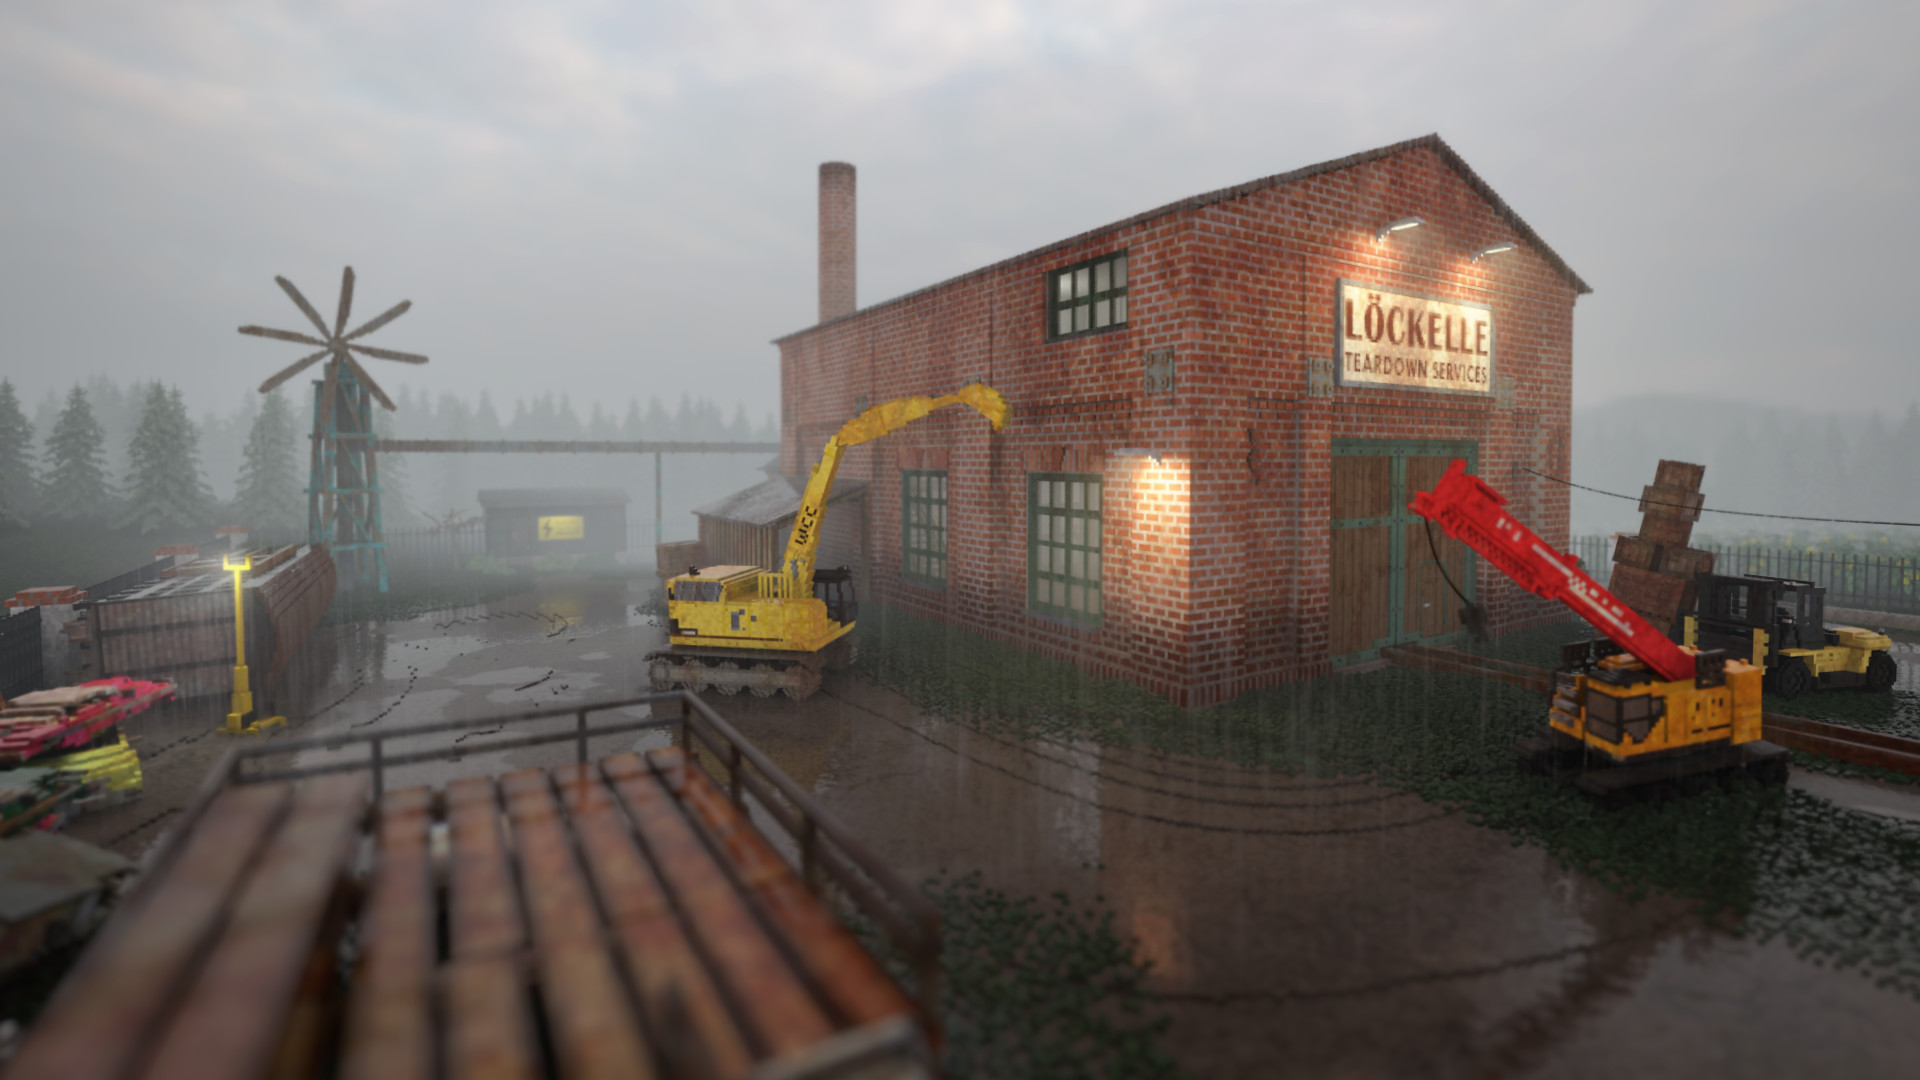
\includegraphics[width=300px]{images/graphics/teardown-ray-tracing.jpg}
    \caption{A screenshot from \emph{Teardown}, showcasing raytraced lighting \cite{TeardownSteam2022}.}
    \label{fig:teardown-raytracing}
\end{figure}

\noindent
During the past years, ray tracing has become a more common rendering technique, being used for global illumination, 
shadows or ambient occlusion in rasterizer pipelines. Fully ray traced real-time rendering has mostly been available 
for voxel rendering, using common optimization techniques like a \ac{BVH}. Voxel data for ray tracing has been a 
major influence for our approach, since their implicit voxel representation is generally compatible with meshes 
generated directly on the \ac{GPU}. Various efforts have been made to optimize voxel representations for ray traced 
pipelines. Kampe et al. \cite{Kampe2013} propose the use of their \emph{High-Resolution Sparse Voxel \ac{DAG}s}, 
as discussed in chapter \ref{subsec-highres-svo-dags}. This approach is tailored to high voxel resolutions and data 
that might not fit into memory all at once. Their data structure can be easily split up into several sub-trees, which 
in turn can be loaded individually. This approach seems promising for large scenes and use cases, which require the 
streaming of data. 


[@TODO: sources]


\section{Occlusion Culling}

In the past, occlusion culling in games has been heavily influenced by \emph{umbra} \cite{Umbra2024}, a company 
specialized on 3D occlusion culling solutions. Umbra has been used by a lot of games such as \emph{Call of Duty: Ghosts} 
(2013), \emph{Killzone: Shadow Fall} (2013), \emph{Alan Wake} (2012) and many more 
\cite{UmbraWiki,CallOfDutyGhostsCredits, KillzoneUmbra,AlanWakeUmbra}. Umbra voxelizes the game world and proceeds 
to process the data further, merging voxels to cells. A runtime hierarchy of the meshes inside the voxelgrid is created 
and subsequently, using the camera position, the cells can be queried for occlusion. As long as there are large 
occluders, this process can reduce the amount of instances and therefore the amount of triangles to draw 
\cite{Bonet2021}. \\

\noindent
\emph{Assassin's Creed Unity} (2014) uses the two-pass occlusion culling discussed in chapter 
\ref{subsubsec-two-pass-occlusion-culling} as presented by Aaltonen et al. \cite{Aaltonen2015}. This technique 
involves both \ac{HZB} and depth reprojection. Both make for a good occlusion culling technique in games with large 
occluders or interiors. It allowed developers to push for huge draw distances and densly crowded environments. The 
game used advanced technology in its implementation. The most similar to our approach being the clustered geometry 
and the \ac{GPU} centric approach of occlusion culling. However, the game doesn't use a volumetric representation but 
the standard boundary representation for its world. \\

\noindent
Similar to \emph{Assassin's Creed Unity}, \emph{Alan Wake 2} (2023) also implements \ac{HZB} and depth reprojection. 
It is directly based on the approach of Aaltonen et al. \cite{Aaltonen2015} but this time makes use of the new mesh 
shading pipeline. The hardware integration of clustering geometry makes this approach even more efficient. \\

\noindent
\emph{Epic Games'} \emph{Unreal Engine 5} also features \ac{HZB}, reprojecting the last frames depth buffer and using 
this data for conservative occlusion culling. This procedure also uses the mesh shading pipeline to cull individual 
meshlets and is significantly influenced by Aaltonen et al. \cite{Aaltonen2015, Karis2021}. 

\noindent [@TODO: Probably remove because its \ac{HZB}]
Another approach of applying occlusion culling is the \emph{raster occlusion culling}, proposed by \emph{NVIDIA}, among 
others \cite{NVIDIAGLOC2016}. The approach relies on "invisibly" rasterizing the objects as bounding boxes and using the 
rasterizer to query visibility checks and storing the per-object results in a visibility buffer. This buffer can then be 
used to draw the actual shaded objects and discard invisible objects. For the bounding boxes, only up to three faces are 
drawn in the early visibility check, to reduce load. Also, this can be optimized using instancing, the geometry shader or 
mesh shading to compute the visibility buffer efficiently \cite{NVIDIAGLOC2016}. This approach, especially when using 
mesh shading, is rather similar to ours. However, our use case is different in a few details.



% SV DAGs
% AC Unity
% Alan Wake 2
% Greene
% 